\documentclass[14pt]{extbook}
\usepackage{multicol, enumerate, enumitem, hyperref, color, soul, setspace, parskip, fancyhdr} %General Packages
\usepackage{amssymb, amsthm, amsmath, bbm, latexsym, units, mathtools} %Math Packages
\everymath{\displaystyle} %All math in Display Style
% Packages with additional options
\usepackage[headsep=0.5cm,headheight=12pt, left=1 in,right= 1 in,top= 1 in,bottom= 1 in]{geometry}
\usepackage[usenames,dvipsnames]{xcolor}
\usepackage{dashrule}  % Package to use the command below to create lines between items
\newcommand{\litem}[1]{\item#1\hspace*{-1cm}\rule{\textwidth}{0.4pt}}
\pagestyle{fancy}
\lhead{Progress Quiz 8}
\chead{}
\rhead{Version C}
\lfoot{4553-3922}
\cfoot{}
\rfoot{Fall 2020}
\begin{document}

\begin{enumerate}
\litem{
Solve the modeling problem below, if possible.
\begin{center}
    \textit{ In CHM2045L, Brittany created a 27 liter 36 percent solution of chemical $\chi$ using two different solution percentages of chemical $\chi$. When she went to write her lab report, she realized she forgot to write the amount of each solution she used! If she remembers she used 7 percent and 36 percent solutions, what was the amount she used of the 36 percent solution? }
\end{center}
\begin{enumerate}[label=\Alph*.]
\item \( 25.23 \)
\item \( 27.00 \)
\item \( 13.50 \)
\item \( -0.00 \)
\item \( \text{There is not enough information to solve the problem.} \)

\end{enumerate} }
\litem{
Determine the appropriate model for the graph of points below.
\begin{center}
    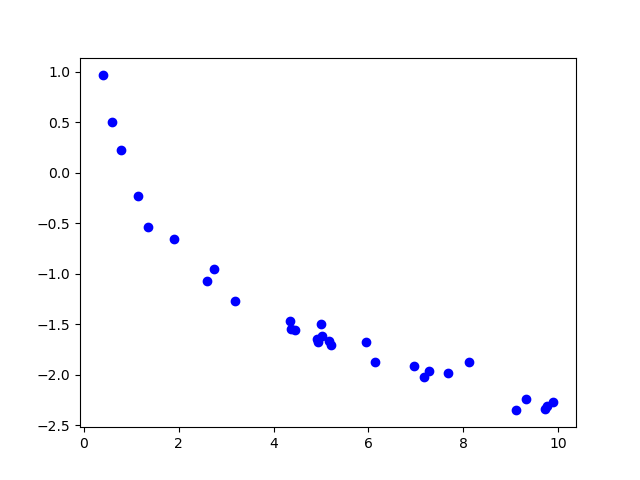
\includegraphics[width=0.5\textwidth]{../Figures/identifyModelGraph12C.png}
\end{center}
\begin{enumerate}[label=\Alph*.]
\item \( \text{Non-linear Power model} \)
\item \( \text{Linear model} \)
\item \( \text{Logarithmic model} \)
\item \( \text{Exponential model} \)
\item \( \text{None of the above} \)

\end{enumerate} }
\litem{
Using the scenario below, model the situation using an exponential function and a base of $\frac{1}{2}$. Then, solve for the half-life of the element, rounding to the nearest day.
\begin{center}
    \textit{ The half-life of an element is the amount of time it takes for the element to decay to half of its initial starting amount. There is initially 577 grams of element $X$ and after 4 years there is 82 grams remaining. }
\end{center}
\begin{enumerate}[label=\Alph*.]
\item \( \text{About } 1825 \text{ days} \)
\item \( \text{About } 365 \text{ days} \)
\item \( \text{About } 730 \text{ days} \)
\item \( \text{About } 0 \text{ days} \)
\item \( \text{None of the above} \)

\end{enumerate} }
\litem{
Determine the appropriate model for the graph of points below.
\begin{center}
    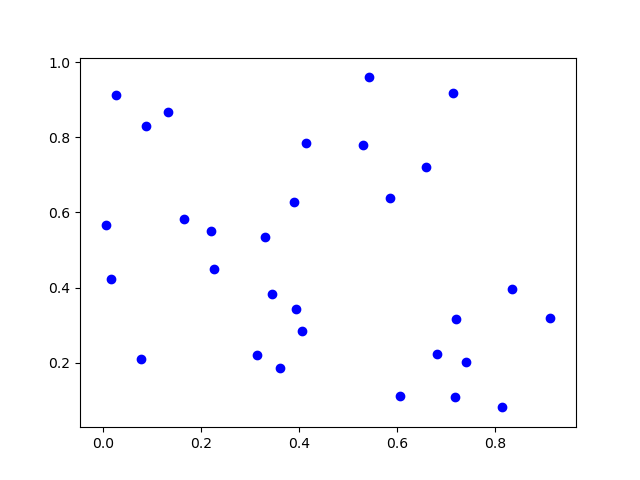
\includegraphics[width=0.5\textwidth]{../Figures/identifyModelGraph12CopyC.png}
\end{center}
\begin{enumerate}[label=\Alph*.]
\item \( \text{Logarithmic model} \)
\item \( \text{Non-linear Power model} \)
\item \( \text{Linear model} \)
\item \( \text{Exponential model} \)
\item \( \text{None of the above} \)

\end{enumerate} }
\litem{
The temperature of an object, $T$, in a different surrounding temperature $T_s$ will behave according to the formula $T(t) = Ae^{kt} + T_s$, where $t$ is minutes, $A$ is a constant, and k is a constant. Use this formula and the situation below to construct a model that describes the uranium's temperature, $T$, based on the amount of time t (in minutes) that have passed. Choose the correct constant $k$ from the options below.
\begin{center}
    \textit{ Uranium is taken out of the reactor with a temperature of $180^{\circ}$ C and is placed into a $11^{\circ}$ C bath to cool. After 17 minutes, the uranium has cooled to $110^{\circ}$ C. }
\end{center}
\begin{enumerate}[label=\Alph*.]
\item \( k = -0.03517 \)
\item \( k = -0.03517 \)
\item \( k = -0.04410 \)
\item \( k = -0.04365 \)
\item \( \text{None of the above} \)

\end{enumerate} }
\litem{
For the scenario below, use the model for the volume of a cylinder as $V = \pi r^2 h$.
\begin{center}
    \textit{ Pringles wants to add 47 \text{percent} more chips to their cylinder cans and minimize the design change of their cans. They've decided that the best way to minimize the design change is to increase the radius and height by the same percentage. What should this increase be? }
\end{center}
\begin{enumerate}[label=\Alph*.]
\item \( \text{About } 24 \text{ percent} \)
\item \( \text{About } 14 \text{ percent} \)
\item \( \text{About } 4 \text{ percent} \)
\item \( \text{About } 21 \text{ percent} \)
\item \( \text{None of the above} \)

\end{enumerate} }
\litem{
Solve the modeling problem below, if possible.
\begin{center}
    \textit{ A new virus is spreading throughout the world. There were initially 4 many cases reported, but the number of confirmed cases has tripled every 5 days. How long will it be until there are at least 10000 confirmed cases? }
\end{center}
\begin{enumerate}[label=\Alph*.]
\item \( \text{About } 40 \text{ days} \)
\item \( \text{About } 19 \text{ days} \)
\item \( \text{About } 36 \text{ days} \)
\item \( \text{About } 20 \text{ days} \)
\item \( \text{There is not enough information to solve the problem.} \)

\end{enumerate} }
\litem{
Solve the modeling problem below, if possible.
\begin{center}
    \textit{ A new virus is spreading throughout the world. There were initially 5 many cases reported, but the number of confirmed cases has quadrupled every 5 days. How long will it be until there are at least 10000 confirmed cases? }
\end{center}
\begin{enumerate}[label=\Alph*.]
\item \( \text{About } 18 \text{ days} \)
\item \( \text{About } 28 \text{ days} \)
\item \( \text{About } 16 \text{ days} \)
\item \( \text{About } 39 \text{ days} \)
\item \( \text{There is not enough information to solve the problem.} \)

\end{enumerate} }
\litem{
For the scenario below, use the model for the volume of a cylinder as $V = \pi r^2 h$.
\begin{center}
    \textit{ Pringles wants to add 31 \text{percent} more chips to their cylinder cans and minimize the design change of their cans. They've decided that the best way to minimize the design change is to increase the radius and height by the same percentage. What should this increase be? }
\end{center}
\begin{enumerate}[label=\Alph*.]
\item \( \text{About } 3 \text{ percent} \)
\item \( \text{About } 9 \text{ percent} \)
\item \( \text{About } 16 \text{ percent} \)
\item \( \text{About } 14 \text{ percent} \)
\item \( \text{None of the above} \)

\end{enumerate} }
\litem{
Solve the modeling problem below, if possible.
\begin{center}
    \textit{ In CHM2045L, Brittany created a 27 liter 26 percent solution of chemical $\chi$ using two different solution percentages of chemical $\chi$. When she went to write her lab report, she realized she forgot to write the amount of each solution she used! If she remembers she used 10 percent and 32 percent solutions, what was the amount she used of the 32 percent solution? }
\end{center}
\begin{enumerate}[label=\Alph*.]
\item \( 14.42 \)
\item \( 13.50 \)
\item \( 19.64 \)
\item \( 7.36 \)
\item \( \text{There is not enough information to solve the problem.} \)

\end{enumerate} }
\end{enumerate}

\end{document}